\chapter{Transactions in hardware: Unbounded Transactional Memory}
\markboth{CHAPTER 6.~~TRANSACTIONS IN HARDWARE: UTM}{}
\label{sec:htm}
\epigraphhead[70]{\epigraph{%
People who are really serious about software should make their own hardware.

Remember, it's all software, it just depends on when you crystallize
it.}{\textit{Alan Kay}}}
\index{Kay, Alan}
% http://www.folklore.org/StoryView.py?project=Macintosh&story=Creative_Think.txt

The previous chapters have detailed the design of an efficient
software-only transaction system for object-oriented programs.  Given
hardware support, we can construct even more efficient transaction
systems for certain types of transactions.  In this chapter, we will
present UTM, an implementation of unbounded transactional memory
\cite{AnanianAsKuLeLi04} which fully virtualizes transactions.  We
will follow this with LTM, a much simpler design which can be
pin-compatible with today's processors.  LTM supports more limited
transactions, but we conclude by showing how LTM can be combined with
the efficient software system we have already demonstrated to yield a
hybrid system with a great deal of power and
flexibility.\footnote{Portions of this section are adapted
from~\cite{AnanianAsKuLeLi04}, co-written with Krste Asanovi\'c,
Bradley C. Kuszmaul, Charles E. Leiserson, and Sean Lie.}

\section{The UTM architecture}\label{sec:utm}
We begin by describing UTM, a system that implements
unbounded transactional memory in hardware.  UTM allows
transactions to grow (nearly) as large as virtual memory.  It also
supports a semantics for nested transactions, where interior
transactions are subsumed into the atomic region represented by the
outer transaction.  Unlike previous schemes that tie a thread's
transactional state to a particular processor and/or cache, UTM
maintains bookkeeping information for a transaction in a
memory-resident data structure, the \defn{transaction log}.  This
enables transactions to survive timeslice interrupts and process
migration from one processor to another.  We first present the
software interface to UTM, and then describe the implementation
details.

\subsection{New instructions}

UTM adds two new instructions to a processor's instruction set
architecture:
\begin{description}
\item[\texttt{XBEGIN pc}:] Begin a new transaction.  The
\texttt{pc} argument to \texttt{XBEGIN} specifies
the address of an \defn{abort handler} (e.g., using a PC-relative offset).
If at any time during the execution of a transaction the hardware determines
that the transaction must fail, it immediately rolls back the
processor and memory state to what it was when \texttt{XBEGIN} was
executed, then jumps to \texttt{pc} to execute the abort handler.
 
\item[\texttt{XEND}:] End the current transaction.  If \texttt{XEND}
completes, then the transaction is committed, and all of its
operations appear to be atomic with respect to any other transaction.
\end{description}

Semantically, we can think of an \texttt{XBEGIN} instruction as a
conditional branch to the abort handler.  The \texttt{XBEGIN} for a
transaction that fails has the behavior of a mispredicted branch.
Initially, the processor executes the \texttt{XBEGIN} as a not-taken
branch, falling through into the body of the transaction.  Eventually
the processor realizes that the transaction cannot commit, at which
point it reverts all processor and memory state back to the point of
misprediction and branches to the abort handler.

In the same manner as our software implementation (\charef{withtrans}),
UTM supports the nesting of transactions by subsuming the inner
transaction.  For example, within an outer transaction, a
subroutine may be called that contains an inner transaction.
UTM simply treats the inner transaction as part of the atomic
region defined by the outer one.  This strategy is correct, because it
maintains the property that the inner transaction executes atomically.
Subsumed nested transactions are implemented by using a counter to
keep track of nesting depth.  If the nesting depth is positive, then
\texttt{XBEGIN} and \texttt{XEND} simply increment and decrement the
counter, respectively, and perform no other transactional bookkeeping.

\subsection{Rolling back processor state}

The branch mispredict mechanism in conventional superscalar processors
can roll back register state only for the small window of recent
instructions that have not graduated from the reorder buffer.  To
circumvent the window-size restriction and allow arbitrary rollback
for unbounded transactions, the processor must be modified to retain
an additional snapshot of the architectural register state.  A UTM
processor saves the state of its architectural registers when it
graduates an \texttt{XBEGIN}\@.  The snapshot is retained either until
the transaction aborts, at which point the snapshot is restored into
the architectural registers, or until the matching \texttt{XEND}
graduates indicating that the transaction has committed.

UTM's modifications to the processor core are illustrated in
\figref{snapshot}.  We assume a machine with a unified physical
register file, and so rather than saving the architectural registers
themselves, UTM saves a snapshot of the register-renaming table
and ensures the corresponding physical registers are not reused until
the transaction commits.
The rename stage maintains an additional ``saved'' bit
for each physical register 
to indicate which registers are part of the working
architectural state, and takes a snapshot as
each branch or \texttt{XBEGIN} is decoded and renamed.
When an \texttt{XBEGIN} instruction
graduates, activating the transaction, the associated ``\texttt{S} bit''
snapshot will have bits set
on exactly those registers holding the graduated architectural state.  Physical
registers are normally freed on graduation of a later instruction that
overwrites the same architectural register.  If the \texttt{S} bit on
the snapshot for the active transaction is
set, the physical register is added to a FIFO called a \defn{Register
Reserved List} instead of the normal \defn{Register Free List}.  This
prevents physical registers containing saved data from being
overwritten during a transaction.  When the
transaction's \texttt{XEND} commits, the active snapshot's \texttt{S}
bits are cleared and the Register
Reserved List is drained into the regular Register Free List.  In the
event that the transaction aborts, the saved register-renaming table
is restored and the reorder buffer is rolled back, as in an exception.
After restoring the architectural register state, the branch is taken
to the abort handler.  Even though the processor can internally
speculatively execute ahead through multiple transactions,
transactions only affect the global memory system as instructions
graduate, and hence UTM requires only a single snapshot of the
architectural register state.

The current transaction abort handler address, nesting depth, and
register snapshot are part of the transactional state.  They are made
visible to the operating system (as additional processor control
registers) to allow them to be saved and restored on context switches.

\subsection{Memory state}

Previous HTM systems \cite{Knight86,HerlihyMo93} represent a
transaction partly in the processor and partly in the cache, taking
advantage of the coincidence between the cache-consistency protocol
and the underlying consistency requirements of transactional memory.
Unlike those systems, UTM transactions are represented by a single
\defn{xstate} data structure held in the memory of the system.  The
cache in UTM is used to gain performance, but the correctness of
UTM does not depend on having a cache.  In the following
paragraphs, we first describe the xstate and how the system uses it
assuming there is no caching.  Then, we describe how caching
accelerates xstate operations.

The xstate is illustrated in \figref{datastruct-entry}.  The xstate
contains a transaction log for each active transaction in the system.
A transaction log is allocated by the operating system for each
thread, and two processor control registers hold the base and bounds
of the currently active thread's log.  Each log consists of a
\defn{commit record} and a vector of \defn{log entries}.  The commit
record maintains the transaction's status: \texttt{PENDING},
\texttt{COMMITTED}, or \texttt{ABORTED}.  Each log entry corresponds
to a block of memory that has been read or written by the transaction.
The entry provides a pointer to the block and the old (backup) value
for the block so that memory can be restored in case the transaction
aborts.  Each log entry also contains a pointer to the commit record
and pointers that form a linked list of all entries in all transaction
logs that refer to the same block.

The final part of the xstate consists of a \defn{log pointer} and one
\defn{RW bit} for each block in memory (and on disk, when paging).  If
the RW bit is \texttt{R}, any transactions that have accessed the
block did so with a load; otherwise, if it is \texttt{W}, the block
may have been the target of a transaction's store.  When a processor
running a transaction reads or writes a block, the block's log pointer
is made to point to a transaction log entry for that block.  Further,
if the access is a write, the RW bit for the block is set to
\texttt{W}.  Whenever another processor references a block that is
already part of a pending transaction, the system consults the RW bit
and log pointer to determine the correct action, for example, to use
the old value, to use the new value, or to abort the transaction.

\figput[UTM processor modifications.]{snapshot}%
{UTM processor modifications. The S bit vector
tracks the active physical registers.  For each rename table snapshot,
there is an associated S bit vector snapshot.  The Register Reserved
List holds the otherwise free physical registers until the transaction
commits.  The LPR field is the next physical register to free (the
last physical register referenced by the destination architectural
register).}

\figput[The xstate data structure.]{datastruct-entry}{%
The xstate data structure.
The transaction log for a transaction contains a commit record and a
vector of log entries.  The log pointer of a block in memory
points to a log entry, which contains the old value of the block and a
pointer to the transaction's commit record.  Two transaction logs
are shown here; generally, the xstate includes the active
transaction logs for the entire system.}

When a processor makes an update as part of a transaction, the new
value is stored in memory and the old value is stored in an entry in
the transaction log.  In principle, there is one log entry for every
load or store performed by the transaction.  If the memory allocated
to the log  is not large enough, the
transaction aborts and the operating system allocates a larger
transaction log and retries the transaction.  When
operating on the same block more than once in a transaction, the
system can avoid writing multiple entries into the transaction log by
checking the log pointer to see whether a log entry for the block
already exists as part of the running transaction.

By following the log pointer to the log entry, then following the log
entry pointer to the commit record, one can determine the transaction
status (pending, committed, or aborted) of each block.  To commit a
transaction, the system simply changes the commit record from
\texttt{PENDING} to \texttt{COMMITTED}.  At this point, a reference to
the block produces the new value stored in memory, albeit after some
delay in chasing pointers to discover that the transaction has been
committed.  To avoid this delay, as well as to free the transaction
log for reuse, the system must clean up after committing.  It does so
by iterating through the log entries, clearing the log pointer for
each block mentioned, thereby finalizing the contents of the block.
Future references to that block will continue to produce the new value
stored in memory, but without the delay of chasing pointers.  To abort
a transaction, the system changes the commit record from
\texttt{PENDING} to \texttt{ABORTED}.  To clean up, it iterates
through the entries, storing the old value back to memory and then
clearing the log pointer.  We chose to store the old value of a block
in the transaction log and the new value in memory, rather than the
reverse, to optimize the case when a transaction commits.  No data
copying is needed to clean up after a commit, only after an abort.

When two or more pending transactions have accessed a block and at
least one of the accesses is a store, the transactions conflict.
Conflicts are detected during operations on memory.  When a
transaction performs a load, the system checks that either the log
pointer refers to an entry in the current transaction log, or else
that the RW bit is \texttt{R} (additionally creating an entry in the
current log for the block if needed).  When a transaction performs a
store, the system checks that no other transaction is referenced by
the log pointer (i.e., that the log pointer is cleared or that the
linked list of log entries corresponding to this block are all
contained in the current transaction log).  If the conflict check
fails, then some of the conflicting transactions are aborted.  To
guarantee forward progress, UTM writes a timestamp into the
transaction log the first time a transaction is attempted.  Then, when
choosing which transactions to abort, older transactions take
priority.  As an alternative, a backoff scheme \cite{MetcalfeBo76}
could also be used.

When a writing transaction wins a conflict, there may be multiple
reading transactions that must be aborted.  These transactions are
found efficiently by following the block's log pointer to an entry and
traversing the linked list found there, which enumerates all entries
for that block in all transaction logs.

\subsection{Caching}

Although UTM can support transactions of unbounded size using the
xstate data structure, multiple memory accesses for each operation may
be required.  Caching is needed to achieve acceptable performance.  In
the common case of a transaction that fits in cache, UTM, like the
earlier proposed HTM systems \cite{Knight86,HerlihyMo93}, monitors the
cache-coherence traffic for the transaction's cache lines to determine
if another processor is performing a conflicting operation.  For
example, when a transaction writes to a memory location, the cache
protocol obtains exclusive ownership on the whole cache block.  New
values can be stored in cache with old values left in memory.  As long
as nothing revokes the ownership of any block, the transaction can
succeed.  Since the contents of the transaction log are undefined
after the transaction commits or aborts, in many cases the system does
not even need to write back a transaction log.  Thus, for a small
transaction that commits without intervention from another
transaction, no additional interprocessor communication is required
beyond the coherence traffic for the nontransactional case.  When the
transaction is too big to fit in cache or interactions with other
transactions are indicated by the cache protocol, the xstate for the
transaction overflows into the ordinary memory hierarchy.  Thus, the
UTM system does not actually need to create a log entry or update
the log pointer for a cached block unless it is evicted.  After a
transaction commits or aborts, the log entries of unspilled cached
blocks can be discarded and the log pointer of each such block can be
marked clean to avoid writeback traffic for the log pointer, which is
no longer needed.  Most of the overhead is borne in the uncommon case,
allowing the common case to run fast.

The in-cache representation of transactional state and the xstate data
structure stored in memory need not match.  The system can optimize
the on-processor representation as long as, at the cache interface, the
view of the xstate is properly maintained.  For convenience, the
transaction block size can match the cache line size.

\subsection{System issues}

The goal of UTM is to support transactions that can run for an
indefinite length of time (surviving time slice interrupts), can
migrate from one processor to another along with the rest of a
process's state, and can have footprints bigger than the physical
memory.  Several system issues must be solved for UTM to achieve that
goal.  The main technique that we propose is to treat the xstate as
a system-wide data structure that uses global virtual addresses.

Treating the xstate as data structure directly solves part of the
problem.  For a transaction to run for an indefinite length of time,
it must be able to survive a time-slice interrupt.  By adding the
log pointer to the processor state and storing everything else in a
data structure, it is easy to suspend a transaction and run another
thread with its own transaction.  Similarly, transactions can be
migrated from one processor to another.  The log pointer is
simply part of the thread or process state provided by the operating
system.

UTM can support transactions that are even larger than physical
memory.  The only limitation is how much virtual memory is available
to store both old and new values.  To page the xstate out of main
memory, the UTM data structures might employ global virtual addresses for
their pointers.  Global virtual addresses are system-wide unique
addresses that remain valid even if the referenced pages are paged out
to disk and reloaded in another location.  Typically, systems that
provide global virtual addresses provide an additional level of
address translation, compared to ordinary virtual memory systems.
Hardware first translates a process's virtual address into a global
virtual address.  The global virtual address is then translated into a
physical address.  Multics \cite{BensoussanClDa72} provided user-level
global virtual addressing using segment-offset pairs as the addresses.
The HP Precision Architecture \cite{Lee89} supports global virtual
addresses in a 64-bit RISC processor.

The log pointer and state bits for each user memory block,
while typically not visible to a user-level programmer, are
themselves stored in addressable physical memory to allow the
operating system to page this information to disk.  The location of
the memory holding the log pointer information for a given user data
page is kept in the page table and cached in the TLB.

During execution of a single load or store instruction, the processor can
potentially touch a large number of disparate memory locations in the
xstate, any of which may be paged out to disk.  To ensure forward
progress, either the system must allow load or store instructions to
be restarted in the middle of the xstate traversal, or, if only
precise interrupts are allowed, the operating system must ensure that
all pages required by an xstate traversal can be resident
simultaneously to allow the load or store to complete without page
faults.

UTM assumes that each transaction is a serial instruction stream
beginning with an \texttt{XBEGIN} instruction, ending with a
\texttt{XEND} instruction, and containing only register, memory, and
branch instructions in between.  A fault occurs if an I/O instruction
is executed during a transaction.

\section{The LTM architecture}\label{sec:ltm}

UTM is an idealized design for HTM that requires significant
changes to both the processor and the memory subsystem of a current
computer architecture.  By scaling back on the degree of
``unboundedness,'' however, a compromise between programmability and
practicality can be achieved.  This section presents such an
architectural compromise, called LTM, for which we have implemented
a detailed cycle-level simulation using UVSIM~\cite{Zhang03}.
The limited transactions supported by LTM are still powerful enough to
serve as the basic for an hybrid system, as we will show in
\charef{hybrid}.

LTM's design is easier to implement than UTM, because it does
not support transactions of virtual-memory size.  Instead, LTM
avoids the intricacies of virtual memory by limiting the footprint of
a transaction to (nearly) the size of physical memory.  In addition,
the duration of a transaction must be less than a time slice and
transactions cannot migrate between processors.  With these
restrictions, LTM can be implemented by only modifying the cache
and processor core and without making changes to the main memory, the
cache-coherence protocols, or even the contents of the cache-coherence
messages.  Unlike a UTM processor, an LTM processor can be
pin-compatible with a conventional processor.  The design presented
here is based on the SGI Origin 3000 shared-memory multiprocessor,
with memory distributed among the processor nodes and cache coherency
maintained using a directory-based write-invalidate protocol.

The UTM and LTM schemes share many ideas.  Like UTM, LTM
maintains data about pending transactions in the cache and detects
conflicts using the cache-coherency protocol in much the same way as
previous HTM proposals~\cite{Knight86, HerlihyMo92}.  LTM also employs an
architectural state-save mechanism in hardware.  Unlike UTM, LTM
does not treat the transaction as a data structure.  Instead, it binds
a transaction to a particular cache.  Transactional data overflows
from the cache into a hash table in main memory, which allows LTM
to handle transactions too big to fit in the cache without the
full implementation complexity of the xstate data structure.

LTM has similar semantics to UTM, and the format and behavior of
the \texttt{XBEGIN} and \texttt{XEND} instructions are the same.
The information that UTM keeps in the transaction log is
kept partly in the processor, partly in the cache, and partly in an
area of physical memory allocated by the operating system.

\figput[LTM cache modifications.]{cachemods}{LTM cache modifications. The T bit indicates if the line is
transactional. The O bit indicates if the set has
overflowed. Overflowed data is stored in a data structure in uncached
DRAM.}

LTM requires only a few small modifications to the cache, as shown
in \figref{cachemods}.  For small transactions, the cache is used to
store the speculative transactional state. For large transactions,
transactional state is spilled into an overflow data structure in main
memory. An additional bit (T) is added per cache line to indicate if
the data has been accessed as part of a pending transaction. When a
transactional-memory request hits a cache line, the T bit is set. An
additional bit (O) is added per cache set to indicate if it has
overflowed. When a transactional cache line is evicted from the cache
for capacity reasons, the O bit is set.

In LTM, the main memory always contains the original state of any
data being modified transactionally, and all speculative transactional
state is stored in the cache and overflow hash table.  A transaction
is committed by simply clearing all the T bits in cache and writing
all overflowed data back to memory. Conflicts are detected using the
cache-coherency protocol.  When an incoming cache intervention hits a
transactional cache line, the running transaction is aborted by simply
clearing all the T bits and invalidating all modified transactional
cache lines.
\note{CSA: I presume we NACK any cache intervention while we're writing
the overflow table back to memory?}

The overflow hash table in uncached main memory is maintained by
hardware, but its location and size are set up by the operating
system.  If a request from the processor or a cache intervention
misses on the resident tags of an overflowed set, the overflow hash
table is searched for the requested line.  If the requested cache line
is found, it is swapped with a line in the cache set and handled like
a hit.  If the line is not found, it is handled like a miss.  While
handling overflows, all incoming cache interventions are stalled using
a NACK-based network protocol.

The LTM overflow data structure uses the low-order bits of the address
as the hash index and uses linear probing to resolve conflicts.  When
the overflow data structure is full, the hardware signals an exception
so that the operating system can increase the size of the hash table
and retry the transaction.

LTM was designed to be a first step towards a truly unbounded
transactional memory system such as UTM.  LTM has most of the
advantages of UTM while being much easier to implement.  As I will
show at the end of the chapter, LTM's
more practical implementation of quasi-unbounded transactional memory
suffices for many real-world concerns, and can be symbiotically paired
with our more flexible software transaction system to achieve truely
unbounded transactions at minimal hardware cost.

%%%%%%%%%%%%%%%%%%%%%%%%%%%%%%%%%%%%%%%%%%%%%%%%%%%%%%%%%5
\section{Optimizing the common case}

A main goal of LTM and UTM is to run the common case fast. As shown in
\secref{htm-benchmarks}, the common case is when transactions are small
and fit in the cache. Therefore, by using the cache and cache
coherency mechanism to handle small transactions, LTM is able to
execute with almost no overhead over serial code in the common
case. In this section, we discuss qualitatively how the LTM
implementation is optimized for the common case and how similar
techniques are used in UTM. The discussion is broken into the
following three cases: starting, running, committing a transaction.

Starting a transaction in LTM requires virtually no overhead in the
common case since the hardware only needs to record the abort handler
address. No communication with the cache or other external hardware is
necessary. There is the added overhead of decoding the \texttt{XBEGIN}
however that overhead is generally insignificant compared to the cost
of the transaction. Further, instruction decode overhead is much lower
in LTM than with locks. Even schemes where the lock is not actually
held such as SLE have higher decode overhead since they have more
instructions. LTM's low transaction startup overhead is a very good
indicator of the corresponding overhead in UTM since transaction start
up in UTM is virtually the same.

Running a transaction in LTM requires no more overhead than running
the corresponding non-synchronized code in the common case. In LTM,
the T bit is simply set on each transactional cache access. LTM's low
overhead in this case unfortunately does not translate directly to UTM
since UTM modifies the transaction record on each memory
request. However, in the common case the transaction record entry is
also in the cache. Thus all operations are local and no external
communication is needed. Also, in some cases, the cache can respond to
the memory request once the requested data is found. However, if the
request requires data from the transaction record before it can be
serviced, an additional cache lookup is necessary. However, the lookup
is local and thus can be done relatively quickly. \note{Is this
enough?  Seems like the additional lookup in the cache could increase
cache latency significantly} Therefore, the common case overhead of
running a transaction can be minimal even in UTM.

Committing a transaction in LTM has virtually no overhead in the
common case since it can be done in one clock cycle. LTM transaction
commits only requires a simply flash clear of all the transaction bits
in the cache. Similarly, UTM transaction commits only require a single
change of the cached transaction record to ``committed''. UTM
transaction commit also writes the updated values from the transaction
record back to memory. However, this write back can be done lazily in
the background.  Therefore, since transaction commit requires only a
single change in the cache for both LTM and UTM, the overhead is
minimal in both cases.

\subsection{Evaluation} % Performance
% overflows -- hey, hybrid scheme!  in hybrid section?
% counter microbenchmark -- hey, we parallelize!

\subsection{Understanding overflows}

Overflows occur only in the uncommon case
however our studies show that it is important to have a scalable data
structure even though it is used infrequently.

For evaluation, we compiled three versions of the SPECjvm98 benchmark
suite to run under UVSIM using our modified Java compiler. We compiled
a \defn{Base} version that uses no synchronization, a \defn{Locks}
version that uses spin-locks for synchronization, and a \defn{Trans}
version that uses LTM transactions for synchronization. To measure
overheads, we ran these versions of the SPECjvm98 benchmark suite on
one processor of UVSIM.

As described in \secref{synctrans}, our transactional version uses method
cloning to flatten transactions; we performed the same cloning on the
other compiled versions so that performance improvements due to the
specialization would not be improperly attributed to
transactionification.  The three different benchmark versions were
built from a common code-base using method inlining in GCC\footnote{We
compiled the files generated by FLEX's ``PreciseC'' backend
(\charef{precisec}) with
\texttt{-O9} for a \texttt{-mips4} target using the
\texttt{n64} API to generate fully-static binaries executable by
UVSIM.}  to remove or replace all invocations of lock and transaction
entry and exit code with appropriate implementations.  No garbage
collection was performed during benchmark runs.


\label{sec:javac}
Our initial results from \charef{efficient} suggested that since
overflows are infrequent, the efficiency of the data structure would
have a negligible effect on overall performance. Therefore, our first
LTM implementation used an unsorted array that required a linear
search on each miss to an overflowed set. The unsorted array was
effective for most of our test cases, as they had less overhead than
locks.  Using LTM with the unsorted array, however, the transactional
version of \texttt{213\_javac} was 14 times slower than the base
version.  Virtually all of the overhead came from handling overflows,
which is not surprising, since the entire application is enclosed in
one large transaction. The large transaction touches 13K cache lines
with 9K lines overflowed.  So, even though only 0.5\% of the
transactional memory operations miss in the cache, each one incurs a
huge search cost. This unexpected slowdown indicated that a naive
unsorted array is insufficient as an overflow data
structure. Therefore, LTM was redesigned to use a hash table to store
overflows.

Since the entire application was enclosed in a transaction, the
\texttt{213\_javac} application was clearly not written to be a
parallel application. However, it is important that an unbounded
transactional memory system be able to support even such applications
with reasonable performance. Therefore, we redesigned LTM to use hash
table as described in \secref{cachemods}.


\begin{figure}
\footnotesize
\begin{center}
\begin{tabular}{l|r|rr|rr}
Benchmark                 &  Base       & Locks         & Trans                  & Time in   & Time in                    \\
application               &  time       & time          & time                   & trans     & overflow                   \\
                          &  (cycles)   & \multicolumn{2}{c|}{(\% of Base time)} & \multicolumn{2}{c}{(\% of Trans time)} \\ \hline
\texttt{200\_check}       &   8.1M      & 124.0\%       & 101.0\%                & 32.5\%     & 0.0085\%                  \\
% \texttt{201\_compress}    & 608.3M      & 102.5\%       & 106.1\%                &  3.8\%     & 4.0\%                     \\
\texttt{202\_jess}        &  75.0M      & 140.9\%       & 108.0\%                & 59.4\%     & 0.0072\%                  \\
\texttt{209\_db}          &  11.8M      & 142.4\%       & 105.2\%                & 54.0\%     & 0\%                       \\
\texttt{213\_javac}       &  30.7M      & 169.9\%       & 114.2\%                & 84.2\%     & 10\%                      \\
\texttt{222\_mpegaudio}   &  99.0M      & 100.3\%       &  99.6\%                &  0.8\%     & 0\%                       \\
\texttt{228\_jack}        & 261.4M      & 175.3\%       & 104.3\%                & 32.1\%     & 0.0056\%                  \\
\end{tabular}
\end{center}
\caption[SPECjvm98 performance on a 1-processor UVSIM simulation.]{%
SPECjvm98 performance on a 1-processor UVSIM simulation.  The {\em
Time in trans} and {\em Time in overflow} are the times spent actually
running a transaction and handling overflows respectively. The input
size is 1. The overflow hash table is 128MB.}
\label{fig:specperf}
\end{figure}

Using LTM with the hash table, the SPECjvm98 application overheads
were much more reasonable as shown in \figref{specperf}.  The hash
table data structure decreased the overhead from a 14x slowdown to
under 15\% in \texttt{213\_javac}. Using the hash table, LTM
transactional overhead is less than locking overhead in all cases.

%%%%%%%%%%%%%%%%%%%%%%%%%%%%%%%%%%%%%%%%%%%%%%
\punt{
These results indicate that UTM will also have minimal overhead, since
the UTM data structure behaves much like the LTM hash table. When we
miss in the cache, LTM requires one additional access of memory to
index the hash table when there is no conflict. Similarly, UTM
requires one additional access of memory to retrieve the requested
cache line.  UTM may require an additional access of memory, however,
to retrieve the transactional record entry. UTM requires at most one
more access to memory than LTM when there is overflow.  Therefore, the
overflow overhead of UTM will be very similar to that of UTM.
}

\subsection{Understanding program behavior}

\begin{figure}
\begin{center}
\begin{tabular}{c}
\includegraphics{Figures/uvsimCounterRuntime}
%% \includegraphics{uvsimLinkedListRuntime.eps}
\end{tabular}
\end{center}
\caption{\texttt{Counter} performance on UVSIM.}
\label{fig:microbenchperf}
\end{figure}

Using LTM we are able to gain insight into how transactional programs
behave in a transactional memory system such as UTM. Using the
\texttt{Counter} microbenchmark, we found that small transactions are
likely to complete even when contention is high. LTM uses the
cache and cache-coherency protocol to store transactional state and
detect conflicts in the common case. Transactional-memory systems that
use the same technique, such as UTM, all exhibit similar
properties for the common case.

We implemented the \texttt{Counter} parallel application to examine
program behavior for small transactions with high contention. Our
results show that the extremely low overhead of small transactions
enable them to almost always complete even when contention is high.

The \texttt{Counter} microbenchmark has one shared variable that each
processor atomically increments repeatedly with no backoff
policy. Each transaction is only a few instructions long and every
processor attempts to write to the same location repeatedly.  Both a
locking and a transactional version of \texttt{Counter} were run on
UVSIM with LTM, and the results are shown in
\figref{microbenchperf}. In the locking version, there is a global
spin-lock that each processor obtains using a
load-linked/store-conditional (LLSC) sequence from the SGI
synchronization libraries.

The locking version scales poorly, because the LLSC causes many cache
interventions even when the lock cannot be obtained. On the other
hand, the transactional version scales much better, despite having no
backoff policy.  When a transaction obtains a cache line, it is likely
to be able to execute a few more instructions before receiving an
intervention since the network latency is high.  Therefore, small
transactions can start and complete (and perhaps even start and
complete the next transaction) before the cache line is taken away.
Similar behavior is expected from UTM since small transactions
effectively use the cache the same way.

%% \subsubsection{The \texttt{LinkedList} microbenchmark}
%% 
%% We implemented the \texttt{LinkedList} parallel application to examine
%% program behavior for moderately sized transactions with varying
%% contention. Our results show that when contention is low, transactions
%% are very efficient as expected. However, as contention increases, the
%% efficiency is highly dependent on the backoff policy. In some cases,
%% simple backoff policies may be insufficient.
%% 
%% The \texttt{LinkedList} application has an equal number of consumer
%% and producer processors. There is one doubly-linked list for each
%% consumer. Each consumers repeatedly takes items from the head of its
%% list while each producer repeatedly adds items to the tail of a random
%% list. The locking version locks the entire list when adding or
%% removing items. Locks are implemented as in \texttt{Counter}.
%% 
%% For very few processors, transactions perform much better than
%% conventional locks because transactions allow concurrent accesses to
%% the head and the tail of the linked list. However, as the number of
%% processors is increased, the chance that multiple producers will
%% conflict increases.  When \texttt{LinkedList} was first implemented,
%% no backoff policy was used and, as a result, livelock prevented
%% program completion for more than two processors. Then,
%% \texttt{LinkedList} was implemented with binary exponential backoff
%% and \figref{microbenchperf} shows those results. Backoff solved the
%% livelock problem however as the contention increases, the performance
%% of the transactions decreases dramatically. At high contention,
%% transactions are being aborted repeatedly and a lot of time is spent
%% in backoff. In fact, for \texttt{LinkedList} after 32 processors the
%% transactional version is slower than the locking version. This
%% suggests that such a simple backoff policy may be insufficient in high
%% contention.
%% 
%% The \texttt{LinkedList} application illustrates the importance of a
%% good back policy in non-obstructive transactional memory systems such
%% as LTM and UTM.  Such systems do not face the problem of
%% deadlock. However, they must prevent livelock using backoff or other
%% policies. Perhaps there needs to be a forward progress guarantee to
%% get reasonable performance in high contention. This is one of the main
%% challenges that transactional memory schemes such as UTM face.
%% 


%%%%%%%%%%%%%%%%%%%%%%%%%%%%%%%%%%%%%%%%%%%%%%%%%%%%%%%%%%%%%%%%%%
%%%%%%%%%%%%%%%%%%%%%%%%%%%%%%%%%%%%%%%%%%%%%%%%%%%%%%%%%%%%%%%%%%
%-----------------------------------------------------------------
%%%%%%%%%%%%%%%%%%%%%%%%%%%%%%%%%%%%%%%%%%%%%%%%%%%%%%%%%%%%%%%%%%
%%%%%%%%%%%%%%%%%%%%%%%%%%%%%%%%%%%%%%%%%%%%%%%%%%%%%%%%%%%%%%%%%%


\section{Evaluation}\label{sec:htm-benchmarks}

\section{Making UTM fast}
% describe how caching works.

% Extending Transactions: beyond atomic power.
\section{Extending hardware transactions}\label{sec:htmplus}
\subsection{Nesting}
\subsection{Exchange and merging}
\subsection{Loopholes and NITs}\label{sec:nit}
\subsection{Opportunistic parallelism}

%%%%%%%%%% Extending the hardware section %%%%%%%%%%555

% First: do we want to?  Next section should how to make software hybrid.

\section{Adding partial rollback}
\subsection{LTM}
% keep a log(n) bit 'nesting level' with each transaction
% bulk decremember nesting level on commit.
% is this really needed?  Why not just 'checkpoints'?
% numbering system: what we really want to do is breadth-first
% numbering of the tree, so that we have well-spaced checkpoints.

\subsection{UTM}
% think about implications here.

\section{Making abort handlers more general}
% calling-convention and function issues.
% save registers in software
% do aborts in software
% this lets us add custom compensation code.
% what environment?  just pick one.

%% Extending Transactions: beyond atomic power.
%\section{Nesting}
%\section{Exchange and merging}
%\section{Loopholes and NITs}\label{sec:nit}
%\section{Opportunistic parallelism}

% LocalWords:  UTM XBEGIN XEND mispredicted misprediction superscalar Herlihy
% LocalWords:  mispredict LTM UVSIM SGI transactionally uncached lookup SPECjvm
% LocalWords:  inlining microbenchmark xstate RW RISC

\section{A Real Implementation}
Some notes about a ``real'' implementation of UTM.

MIPS.  Let's assume a primary cache line of 16 bytes, and a secondary
cache line of 128 bytes.  Our transaction block size will be the same
as the secondary cache line size, 128-bytes, which will limit our
address-space overhead to approximately 8\%.  The transaction data (descriptor)
associated with a block will fit into 8 bytes (one 64-bit word), since
virtual addresses are limited to 40 bits on MIPS (42 if you include
the kernel/supervisor/user mode bits; AMD-64 has 52-bit virtual
addresses).\footnote{A(63:62)=$10_2$ is not currently used; we could
steal this to indicate ``transaction descriptors''.  This would probably
cause protection problems.}

There would be 16 transaction descriptor words on a cache line; this
could cause ping-ponging.  An 8k page contains descriptors for the
transaction blocks on 16 other pages ($2^{10}$ descriptors).  The
descriptors should be arranged so the ``no information'' is an
all-zeros pattern.  The OS can then garbage collect any transaction
descriptor pages which contain all zeros (instead of eg paging them to
disk; I believe most OSes will do this optimization already, but maybe
not if the page was once dirty).\footnote{Alternatively, we could reference
count these pages in the page table, and deallocate them when the
number of non-zero entries on the page drops to zero.  This is
probably not the best way to do it.}

To find the transaction descriptor for a given virtual address, we
just flip a high-order bit and shift the low-order bits.  This reuses
the TLB, etc, mechanisms for virtualization, but we must be careful
that we can still ensure forward progress and don't introduce spurious
transaction performance conflicts (because transaction descriptors for
two different transactions reside on the same cache line).

The caches need to know the details of these 'special' addresses so
that ``on chip'' transactions are handled correctly.  In fact, the
cache organization would probably look more like the figure (with the
information stored alongside the cache lines), and we might want to
have extra cache-associativity or other mechanisms to prevent
ping-ponging of the transaction descriptors. (Is this right?)

Nice feature: pin-compatible UTM!  Only the processor and caches
(maybe not even the L2 cache) need to know about transactions.
May be nice to have a word-level caching strategy.

Nice idea (with Bradley): so one concern is that a neighboring xaction
(in the same 2k memory block) may need to access a transaction
descriptor on the same cache line as our transaction descriptor.  We
can handle this by (ahead of time) obtaining the 'next' line in our
transaction log w/ exclusive access.  When we need to ship the cache
line with our descriptor, we just write in the address of the 'next'
log line.  We can then fill this with appropriate information in our
cache, but we still don't actually have to write it back out into main
memory unless someone actually tries to follow the pointer (in which
case we're likely to conflict anyway).  We may want to hack the cache
coherence protocol slightly to allow us exclusive access to a large
log region, which we can generate data for on-the-fly if need be.
This solves the problem where we have to spill our transaction just
because another transaction occurred in the same 2k block.

Another alternative: 9-bit bytes would give enough transaction
descriptor info for 64-byte transaction blocks.




\section{A hybrid transaction implementation}\label{sec:hybrid}
\section{A hybrid transaction implementation}\label{sec:hybrid}

\begin{figure}[t]\begin{center}%
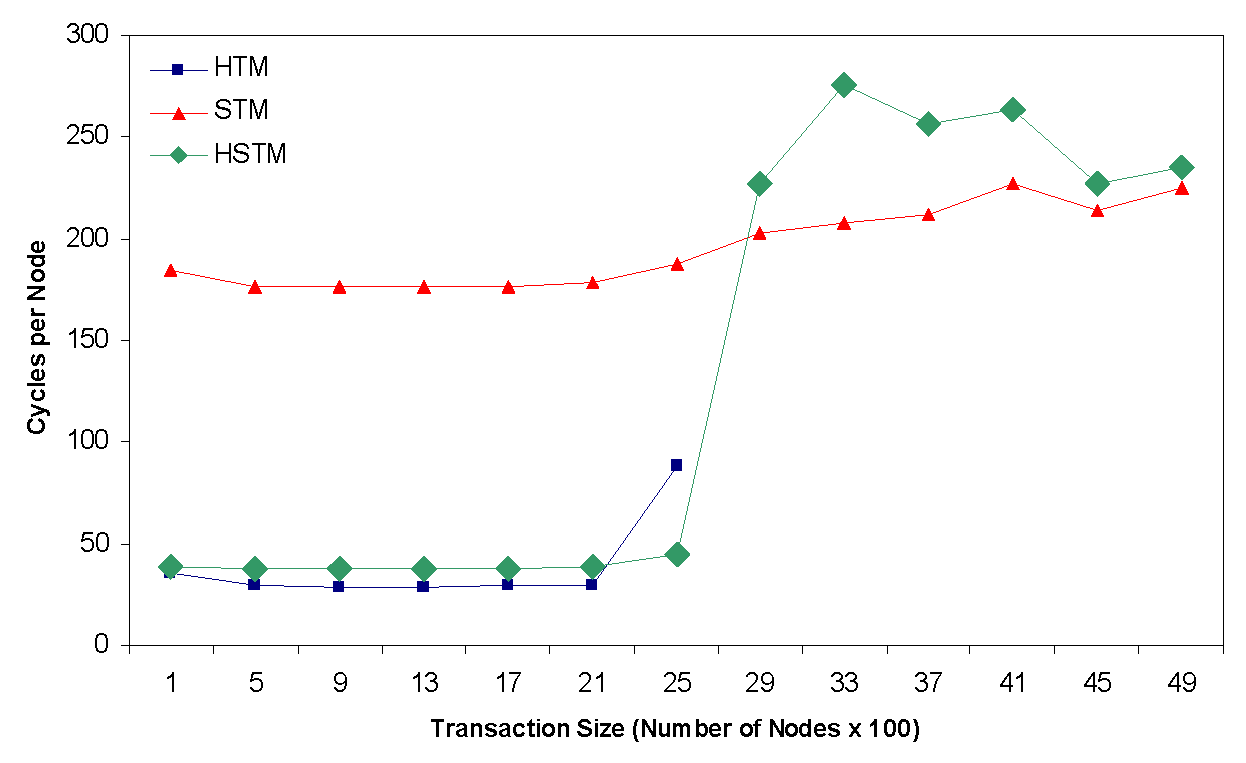
\includegraphics[width=3.25in,clip=true]{Figures/sean_lie_6b}%
\end{center}%
\caption[Hybrid performance on simple queue benchmark.]
{Performance (in cycles per node push on a simple queue
  benchmark) of LTM~\cite{AnanianAsKuLeLi04} (HTM), the
  object-based system presented in this paper (STM) and a hybrid
  scheme (HSTM).}%
\label{fig:hybrid}%
\end{figure}
It is worth considering if a low-level HTM can yield benefits other
than efficient implementations of large-object operations.  In fact,
\figref{hybrid} presents research showing that we can combine the
strengths of our object-based software transaction system with a
fast bounded-size HTM.  In the figure, combining the systems is done
in the most simple-minded way: all transactions are begun in
LTM~\cite{AnanianAsKuLeLi04},
and after any abort the transaction is restarted in the
object-based software system.
  The field flag mechanism described in
\secref{flagfield} ensures that software transactions properly abort
conflicting hardware transactions --- when the software scribbles
\FLAG over the original field the hardware will detect the conflict.
Hardware transactions must perform
the \texttt{ReadNT} and \texttt{WriteNT} algorithms to ensure they
interact properly with concurrent software transactions, although these
checks can be done in software (they do not need to be part of the
hardware HTM mechanism).  In the figure, the read barriers were done
in software, and caused a 2.2x slowdown for the (very small) hardware
transactions.  This is a pessimistic figure: no special effort was
made to tune code or otherwise minimize slowdown, and the processor
simulated had limited ability to exploit ILP (2 ALUs and 4-instruction
issue width).  Even so, the read barriers might be a worthwhile target
for hardware support \cite{ClickTeWo05}.

As a fortuitous synergy, hardware support for small transactions may
also be used to implement the software transaction implementation's
Load Linked/Store Conditional sequences, which may not
otherwise be available on a target processor.

